\documentclass{beamer}

\usepackage[utf8x]{inputenc}
\usepackage{fancyvrb}
\usepackage{color}
\usepackage{graphicx}

\usetheme{Darmstadt}

\title {Code Coverage and the Definition of Done}
\author{Dénes Mátételki}
\institute{www.emerson.com}
\date{October 2, 2012}

\makeatletter
\def\PY@reset{\let\PY@it=\relax \let\PY@bf=\relax%
    \let\PY@ul=\relax \let\PY@tc=\relax%
    \let\PY@bc=\relax \let\PY@ff=\relax}
\def\PY@tok#1{\csname PY@tok@#1\endcsname}
\def\PY@toks#1+{\ifx\relax#1\empty\else%
    \PY@tok{#1}\expandafter\PY@toks\fi}
\def\PY@do#1{\PY@bc{\PY@tc{\PY@ul{%
    \PY@it{\PY@bf{\PY@ff{#1}}}}}}}
\def\PY#1#2{\PY@reset\PY@toks#1+\relax+\PY@do{#2}}

\expandafter\def\csname PY@tok@gd\endcsname{\def\PY@tc##1{\textcolor[rgb]{0.63,0.00,0.00}{##1}}}
\expandafter\def\csname PY@tok@gu\endcsname{\let\PY@bf=\textbf\def\PY@tc##1{\textcolor[rgb]{0.50,0.00,0.50}{##1}}}
\expandafter\def\csname PY@tok@gt\endcsname{\def\PY@tc##1{\textcolor[rgb]{0.00,0.25,0.82}{##1}}}
\expandafter\def\csname PY@tok@gs\endcsname{\let\PY@bf=\textbf}
\expandafter\def\csname PY@tok@gr\endcsname{\def\PY@tc##1{\textcolor[rgb]{1.00,0.00,0.00}{##1}}}
\expandafter\def\csname PY@tok@cm\endcsname{\let\PY@it=\textit\def\PY@tc##1{\textcolor[rgb]{0.25,0.50,0.50}{##1}}}
\expandafter\def\csname PY@tok@vg\endcsname{\def\PY@tc##1{\textcolor[rgb]{0.10,0.09,0.49}{##1}}}
\expandafter\def\csname PY@tok@m\endcsname{\def\PY@tc##1{\textcolor[rgb]{0.40,0.40,0.40}{##1}}}
\expandafter\def\csname PY@tok@mh\endcsname{\def\PY@tc##1{\textcolor[rgb]{0.40,0.40,0.40}{##1}}}
\expandafter\def\csname PY@tok@go\endcsname{\def\PY@tc##1{\textcolor[rgb]{0.50,0.50,0.50}{##1}}}
\expandafter\def\csname PY@tok@ge\endcsname{\let\PY@it=\textit}
\expandafter\def\csname PY@tok@vc\endcsname{\def\PY@tc##1{\textcolor[rgb]{0.10,0.09,0.49}{##1}}}
\expandafter\def\csname PY@tok@il\endcsname{\def\PY@tc##1{\textcolor[rgb]{0.40,0.40,0.40}{##1}}}
\expandafter\def\csname PY@tok@cs\endcsname{\let\PY@it=\textit\def\PY@tc##1{\textcolor[rgb]{0.25,0.50,0.50}{##1}}}
\expandafter\def\csname PY@tok@cp\endcsname{\def\PY@tc##1{\textcolor[rgb]{0.74,0.48,0.00}{##1}}}
\expandafter\def\csname PY@tok@gi\endcsname{\def\PY@tc##1{\textcolor[rgb]{0.00,0.63,0.00}{##1}}}
\expandafter\def\csname PY@tok@gh\endcsname{\let\PY@bf=\textbf\def\PY@tc##1{\textcolor[rgb]{0.00,0.00,0.50}{##1}}}
\expandafter\def\csname PY@tok@ni\endcsname{\let\PY@bf=\textbf\def\PY@tc##1{\textcolor[rgb]{0.60,0.60,0.60}{##1}}}
\expandafter\def\csname PY@tok@nl\endcsname{\def\PY@tc##1{\textcolor[rgb]{0.63,0.63,0.00}{##1}}}
\expandafter\def\csname PY@tok@nn\endcsname{\let\PY@bf=\textbf\def\PY@tc##1{\textcolor[rgb]{0.00,0.00,1.00}{##1}}}
\expandafter\def\csname PY@tok@no\endcsname{\def\PY@tc##1{\textcolor[rgb]{0.53,0.00,0.00}{##1}}}
\expandafter\def\csname PY@tok@na\endcsname{\def\PY@tc##1{\textcolor[rgb]{0.49,0.56,0.16}{##1}}}
\expandafter\def\csname PY@tok@nb\endcsname{\def\PY@tc##1{\textcolor[rgb]{0.00,0.50,0.00}{##1}}}
\expandafter\def\csname PY@tok@nc\endcsname{\let\PY@bf=\textbf\def\PY@tc##1{\textcolor[rgb]{0.00,0.00,1.00}{##1}}}
\expandafter\def\csname PY@tok@nd\endcsname{\def\PY@tc##1{\textcolor[rgb]{0.67,0.13,1.00}{##1}}}
\expandafter\def\csname PY@tok@ne\endcsname{\let\PY@bf=\textbf\def\PY@tc##1{\textcolor[rgb]{0.82,0.25,0.23}{##1}}}
\expandafter\def\csname PY@tok@nf\endcsname{\def\PY@tc##1{\textcolor[rgb]{0.00,0.00,1.00}{##1}}}
\expandafter\def\csname PY@tok@si\endcsname{\let\PY@bf=\textbf\def\PY@tc##1{\textcolor[rgb]{0.73,0.40,0.53}{##1}}}
\expandafter\def\csname PY@tok@s2\endcsname{\def\PY@tc##1{\textcolor[rgb]{0.73,0.13,0.13}{##1}}}
\expandafter\def\csname PY@tok@vi\endcsname{\def\PY@tc##1{\textcolor[rgb]{0.10,0.09,0.49}{##1}}}
\expandafter\def\csname PY@tok@nt\endcsname{\let\PY@bf=\textbf\def\PY@tc##1{\textcolor[rgb]{0.00,0.50,0.00}{##1}}}
\expandafter\def\csname PY@tok@nv\endcsname{\def\PY@tc##1{\textcolor[rgb]{0.10,0.09,0.49}{##1}}}
\expandafter\def\csname PY@tok@s1\endcsname{\def\PY@tc##1{\textcolor[rgb]{0.73,0.13,0.13}{##1}}}
\expandafter\def\csname PY@tok@sh\endcsname{\def\PY@tc##1{\textcolor[rgb]{0.73,0.13,0.13}{##1}}}
\expandafter\def\csname PY@tok@sc\endcsname{\def\PY@tc##1{\textcolor[rgb]{0.73,0.13,0.13}{##1}}}
\expandafter\def\csname PY@tok@sx\endcsname{\def\PY@tc##1{\textcolor[rgb]{0.00,0.50,0.00}{##1}}}
\expandafter\def\csname PY@tok@bp\endcsname{\def\PY@tc##1{\textcolor[rgb]{0.00,0.50,0.00}{##1}}}
\expandafter\def\csname PY@tok@c1\endcsname{\let\PY@it=\textit\def\PY@tc##1{\textcolor[rgb]{0.25,0.50,0.50}{##1}}}
\expandafter\def\csname PY@tok@kc\endcsname{\let\PY@bf=\textbf\def\PY@tc##1{\textcolor[rgb]{0.00,0.50,0.00}{##1}}}
\expandafter\def\csname PY@tok@c\endcsname{\let\PY@it=\textit\def\PY@tc##1{\textcolor[rgb]{0.25,0.50,0.50}{##1}}}
\expandafter\def\csname PY@tok@mf\endcsname{\def\PY@tc##1{\textcolor[rgb]{0.40,0.40,0.40}{##1}}}
\expandafter\def\csname PY@tok@err\endcsname{\def\PY@bc##1{\setlength{\fboxsep}{0pt}\fcolorbox[rgb]{1.00,0.00,0.00}{1,1,1}{\strut ##1}}}
\expandafter\def\csname PY@tok@kd\endcsname{\let\PY@bf=\textbf\def\PY@tc##1{\textcolor[rgb]{0.00,0.50,0.00}{##1}}}
\expandafter\def\csname PY@tok@ss\endcsname{\def\PY@tc##1{\textcolor[rgb]{0.10,0.09,0.49}{##1}}}
\expandafter\def\csname PY@tok@sr\endcsname{\def\PY@tc##1{\textcolor[rgb]{0.73,0.40,0.53}{##1}}}
\expandafter\def\csname PY@tok@mo\endcsname{\def\PY@tc##1{\textcolor[rgb]{0.40,0.40,0.40}{##1}}}
\expandafter\def\csname PY@tok@kn\endcsname{\let\PY@bf=\textbf\def\PY@tc##1{\textcolor[rgb]{0.00,0.50,0.00}{##1}}}
\expandafter\def\csname PY@tok@mi\endcsname{\def\PY@tc##1{\textcolor[rgb]{0.40,0.40,0.40}{##1}}}
\expandafter\def\csname PY@tok@gp\endcsname{\let\PY@bf=\textbf\def\PY@tc##1{\textcolor[rgb]{0.00,0.00,0.50}{##1}}}
\expandafter\def\csname PY@tok@o\endcsname{\def\PY@tc##1{\textcolor[rgb]{0.40,0.40,0.40}{##1}}}
\expandafter\def\csname PY@tok@kr\endcsname{\let\PY@bf=\textbf\def\PY@tc##1{\textcolor[rgb]{0.00,0.50,0.00}{##1}}}
\expandafter\def\csname PY@tok@s\endcsname{\def\PY@tc##1{\textcolor[rgb]{0.73,0.13,0.13}{##1}}}
\expandafter\def\csname PY@tok@kp\endcsname{\def\PY@tc##1{\textcolor[rgb]{0.00,0.50,0.00}{##1}}}
\expandafter\def\csname PY@tok@w\endcsname{\def\PY@tc##1{\textcolor[rgb]{0.73,0.73,0.73}{##1}}}
\expandafter\def\csname PY@tok@kt\endcsname{\def\PY@tc##1{\textcolor[rgb]{0.69,0.00,0.25}{##1}}}
\expandafter\def\csname PY@tok@ow\endcsname{\let\PY@bf=\textbf\def\PY@tc##1{\textcolor[rgb]{0.67,0.13,1.00}{##1}}}
\expandafter\def\csname PY@tok@sb\endcsname{\def\PY@tc##1{\textcolor[rgb]{0.73,0.13,0.13}{##1}}}
\expandafter\def\csname PY@tok@k\endcsname{\let\PY@bf=\textbf\def\PY@tc##1{\textcolor[rgb]{0.00,0.50,0.00}{##1}}}
\expandafter\def\csname PY@tok@se\endcsname{\let\PY@bf=\textbf\def\PY@tc##1{\textcolor[rgb]{0.73,0.40,0.13}{##1}}}
\expandafter\def\csname PY@tok@sd\endcsname{\let\PY@it=\textit\def\PY@tc##1{\textcolor[rgb]{0.73,0.13,0.13}{##1}}}

\def\PYZbs{\char`\\}
\def\PYZus{\char`\_}
\def\PYZob{\char`\{}
\def\PYZcb{\char`\}}
\def\PYZca{\char`\^}
\def\PYZam{\char`\&}
\def\PYZlt{\char`\<}
\def\PYZgt{\char`\>}
\def\PYZsh{\char`\#}
\def\PYZpc{\char`\%}
\def\PYZdl{\char`\$}
\def\PYZti{\char`\~}
% for compatibility with earlier versions
\def\PYZat{@}
\def\PYZlb{[}
\def\PYZrb{]}


\makeatother

\begin{document}

%----------- slide --------------------------------------------------%

\begin{frame}
\titlepage
\end{frame}

%----------- slide --------------------------------------------------%

\begin{frame}
\frametitle{Table of contents}
\tableofcontents
\end{frame}

%----------- slide --------------------------------------------------%

\section{Definitions}

\subsection{Testing}

%----------- slide --------------------------------------------------%

\begin{frame}{Testing}

\begin{block}{Legacy code}
\small
"Code without tests is bad code. It doesn't matter how well written it is; it doesn't matter how pretty or object-oriented or well-encapsulated it is. With tests, we can change the behaviour of our code quickly and verifiably. Without them, we really don't know if our code is getting better or worse." \cite{legacy}
\end{block}

\begin{block}{Unit Test (UT) - white box testing}
\small
"The goal of unit testing is to isolate each part of the program and show that the individual parts are correct. A unit test provides a strict, written contract that the piece of code must satisfy." \cite{ut}
\end{block}

\begin{block}{Functional Test (FT) - black box testing}
\small
"Bases its test cases on the specifications of the software component under test. Functions are tested by feeding them input and examining the output, and internal program structure is rarely considered." \cite{ft}
\end{block}

\end{frame}

%----------- slide --------------------------------------------------%

\begin{frame}{Testing}

\begin{block}{Definition of Done (DoD)}
\small
\begin{itemize}
  \item "A checklist of valuable activities required to produce software." \cite{dod}
  \item "Writing code, coding comments, unit testing, integration testing, release notes, design documents, etc"
  \item "Different DoD at various levels: feature, sprint, release."
  \item Each team come up with their own DoD which is reviewed and updated as needed.
  \item Example: unit tests cover >90% lines of the code
\end{itemize}
\end{block}

\begin{block}{Continuous Integration (CI)}
\small
"Implements continuous processes of applying quality control - small pieces of effort, applied frequently." \cite{ci}

\begin{itemize}
  \item Automate the build
  \item Make the build self-testing
  \item Everyone can see the results of the latest build
  \item ...verifies DOD.
\end{itemize}
\end{block}

\end{frame}

%----------- slide --------------------------------------------------%

\begin{frame}{gcov and gprof}

\begin{block}{gcov}
\small
"gcov is a tool you can use in conjunction with GCC to test code coverage in your programs." \cite{gcov}

\begin{itemize}
  \item how often each line of code executes
  \item which lines of code are actually executed
\end{itemize}
\end{block}

\begin{block}{gprof}
\small
The GNU profiler. \cite{gprof}

\begin{itemize}
  \item how much computing time each section of code uses.
\end{itemize}
\end{block}

\end{frame}


%----------- slide --------------------------------------------------%

\begin{frame}{how gcov works}

\begin{block}{how gcov works}
\small

\begin{itemize}
  \item "The .gcno notes file is generated when the source file is compiled with the GCC -ftest-coverage option. It contains information to reconstruct the basic block graphs and assign source line numbers to blocks."
  \item "The .gcda count data file is generated when a program containing object files built with the GCC -fprofile-arcs option is executed. A separate .gcda file is created for each object file compiled with this option. It contains arc transition counts, value profile counts, and some summary information."
\end{itemize}
\end{block}

\end{frame}

%----------- slide --------------------------------------------------%

\begin{frame}{example}

\begin{block}{sample c code}
\small

#include <stdio.h>

int main (void)
{
  int i, total;

  total = 0;

  for (i = 0; i < 10; i++)
    total += i;

  if (total != 45)
    printf ("Failure\n");
  else
    printf ("Success\n");
  return 0;
}

$ gcc -fprofile-arcs -ftest-coverage tmp.c
$ a.out

gcov

$ gcov tmp.c
File 'tmp.c'
Lines executed:87.50% of 8
tmp.c:creating 'tmp.c.gcov'


$cat tmp.c.gcov

        -:    0:Source:tmp.c
        -:    0:Graph:tmp.gcno
        -:    0:Data:tmp.gcda
        -:    0:Runs:1
        -:    0:Programs:1
        -:    1:#include <stdio.h>
        -:    2:
        1:    3:int main (void)
        -:    4:{
        -:    5:  int i, total;
        -:    6:
        1:    7:  total = 0;
        -:    8:
       11:    9:  for (i = 0; i < 10; i++)
       10:   10:    total += i;
        -:   11:
        1:   12:  if (total != 45)
    #####:   13:    printf ("Failure\n");
        -:   14:  else
        1:   15:    printf ("Success\n");
        1:   16:  return 0;
        -:   17:}
\end{block}

\end{frame}

%----------- slide --------------------------------------------------%

\begin{frame}{how gcov works}

\begin{block}{note}
\small

\begin{itemize}
  \item You can combine the results of many runs into one gcda data.
  \item UTs' and FTs' results can be combined.
\end{itemize}
\end{block}

\end{frame}

\begin{block}{note}
\small

\begin{itemize}
  \item "You should compile your code without optimization." - "optimizer can eliminate some simple code lines by combining them with other lines"
  \item "It works best with a programming style that uses only one statement per line."
  \item "Inlineable functions can create unexpected line counts."
\end{itemize}
\end{block}

\end{frame}

%----------- slide --------------------------------------------------%

\begin{frame}{lcov}

\begin{block}{lcov}
\small
"LCOV is a graphical front-end for GCC's coverage testing tool gcov. It collects gcov data for multiple source files and creates HTML pages containing the source code annotated with coverage information. It also adds overview pages for easy navigation within the file structure." \cite{lcov}
\end{block}

\end{frame}

\begin{block}{asdasd}
$ gcc -fprofile-arcs -ftest-coverage tmp.c
$ a.out
$ lcov --directory . --capture -o lcov.info
$ mkdir cov
$ genhtml --frames --legend  --function-coverage  --branch-coverage  --highlight --demangle-cpp  -o ./cov lcov.info
\end{block}

\end{frame}

%----------- slide --------------------------------------------------%

\begin{frame}{lcov picture 1}

\begin{center}
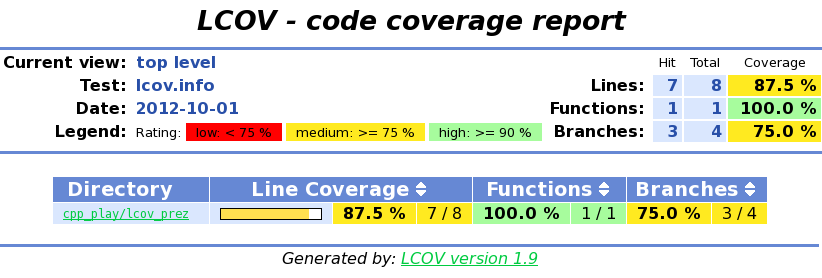
\includegraphics[height=5cm]{tmp.c_lcov_overview.png}
\end{center}

\end{frame}

%----------- slide --------------------------------------------------%

\begin{frame}{lcov picture 2}

\begin{center}
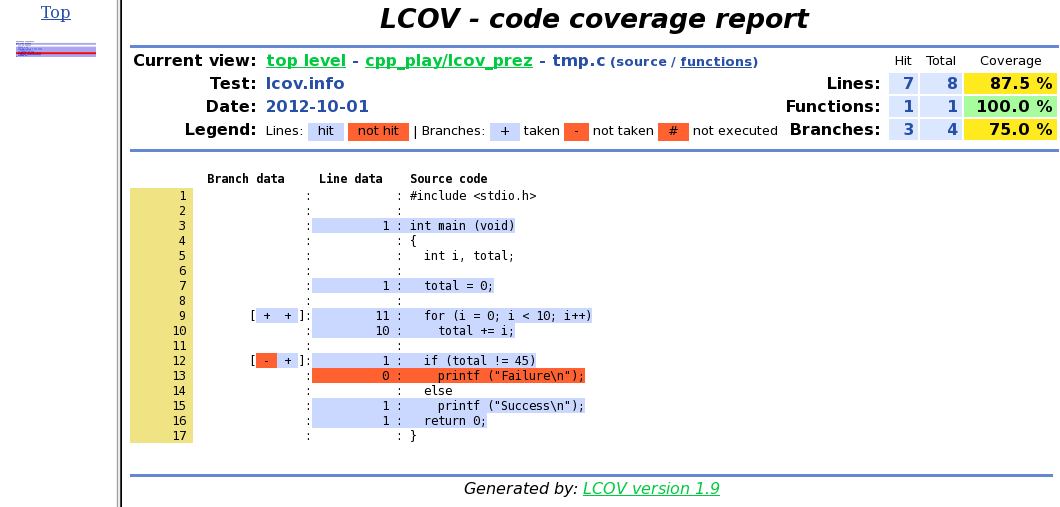
\includegraphics[height=5cm]{tmp.c_lcov_source.png}
\end{center}

\end{frame}

%----------- slide --------------------------------------------------%

\begin{frame}{lcov picture 2}

What we actually got:

 + how often each line of code executes
 + what lines of code are actually executed

But! Line testing is not funtionality testing

 - UTs report code correctness.
 - CC reports...UT correctness?

It's easy to write meaningless UTs to raise CC.
UTs should cover functionality.
Without understanding the UTs, all we can get from CC is:

 + Discovering untested parts.
 + Detecting dead code.

\end{frame}

%----------- slide --------------------------------------------------%

\begin{frame}{final thoughs}

\begin{block}{Testing}
\small

\begin{itemize}
  \item FTs can be written by a "test team" which is sometimes the specification team.
  \item UTs can be written with Test Driven Development - TDD \cite{tdd}
  \item Test and code writer better be a different person otherwise if the code writer misunderstood the requirement, he tests his false model.
  \item Review tests, not just code.
  \item Test code quality should meet the same level as code quality.
  \item Test plan.
  \item Test documentation.
\end{itemize}
\end{block}

\begin{block}{Code coverage as a part of DoD}
\small

\begin{itemize}
  \item The team agrees on testing principles.
  \item Code coverage can be >X%
  \item This rule can be enforced by CI: build fails if CC<X%.
\end{itemize}
\end{block}

\end{frame}

%----------- slide --------------------------------------------------%

\begin{frame}{Links}

\begin{center}
\includegraphics[height=5cm]{qr_code.png}
\end{center}


\tiny
\begin{thebibliography}{100}

\bibitem{legacy}
Michael C. Feathers, \emph{Working Effectively with Legacy Code} Prentice Hall, 2004 ISBN 0-13-117705-2

\bibitem{ut}
Kolawa, Adam; Huizinga, Dorota (2007). \emph{Automated Defect Prevention: Best Practices in Software Management} Wiley-IEEE Computer Society Press. p. 426. ISBN 0-470-04212-5.

\bibitem{ft}
Kaner, Falk, Nguyen. \emph{Testing Computer Software} Wiley Computer Publishing, 1999, p. 42. ISBN 0-471-35846-0.

\bibitem{dod}
http://www.scrumalliance.org/articles/105-what-is-definition-of-done-dod

\bibitem{ci}
http://en.wikipedia.org/wiki/Continuous_integration

\bibitem{gcov}
http://gcc.gnu.org/onlinedocs/gcc/Gcov.html

\bibitem{gprof}
http://www.cs.utah.edu/dept/old/texinfo/as/gprof_toc.html

\bibitem{lcov}
http://ltp.sourceforge.net/coverage/lcov.php

\bibitem{tdd}
http://en.wikipedia.org/wiki/Test-driven_development

\end{thebibliography}
\end{frame}

%----------- slide --------------------------------------------------%

\end{document}
